% !TeX root = RJwrapper.tex
\title{IVYplot: Enhancing a Dot Plot by Representing Observations as Leaflets}
\author{by Tri Nguyen, Mamunur Rashid, and Jyotirmoy Sarkar}

\maketitle

\abstract{%
For a large data set, a dot plot poses a challenge---albeit
unintended---in counting the dots. To overcome this shortcoming Sarkar
and Rashid (2021) proposed an IVY plot, which represents tied data in
batches of five by depicting an IVY leaf with five leaflets. These
leaves are bottom-justified and stacked vertically, with the topmost
leaf possibly having fewer than five leaflets, until the number of
leaflets equals the frequency at each value.
}

\hypertarget{introduction}{%
\subsection{Introduction}\label{introduction}}

A dot plot (Wilkinson, 1999) is commonly used to represent univariate
data without distortion. However, when the data size is large, say
several hundred observations, the accumulated dots may be hard to count
quickly. Sarkar and Rashid (2021) proposed an IVY plot to overcome this
shortcoming. The objective of this paper is to explain step-by-step how
the package IVYplot implements the proposal to draw an IVY plot. After
reading this paper, readers will be equipped to construct an IVY plot
for any data set. They also have some flexibility in modifying the
recommended default plot.

The output of the package IVYplot is a graph that depicts each
observation as a leaflet. Five leaflets are assembled to form a leaf
resembling that of an ivy plant. These leaves are bottom-justified and
stacked vertically, with the topmost leaf possibly having fewer than
five leaflets, until the number of leaflets equals the frequency at each
value. If the frequency at a value exceeds one hundred, we allow each
leaf to represent multiple observations, which number is printed in the
subtitle. Additionally, to ease counting the leaves fast, we add a small
vertical space after every string of five leaves.

\hypertarget{the-ivyplot-package}{%
\subsection{The IVYplot Package}\label{the-ivyplot-package}}

The IVYplot function takes in 8 arguments, with only one argument
mandatory.

\begin{verbatim}
data
\end{verbatim}

A vector of observations for which to make an IVY Plot. This is
mandatory.

\begin{verbatim}
showFreq
\end{verbatim}

Logical. The user can choose TRUE/FALSE to show/not show the exact
frequency at each value. This is especially useful if at least one value
has a frequency exceeding 100, causing each leaflet to represent \(m>1\)
observations. Since the topmost leaflet may represent
\(1,\ 2,\ \ldots,\ m\) observations, the display of the exact
frequencies removes any ambiguity. The default value for this argument
is TRUE.

\begin{verbatim}
freqSize
\end{verbatim}

The user can choose the font size of the frequencies printed under the
vertical stacks of leaves. The default font size is 1.0.

\begin{Schunk}
\begin{figure}[htbp]

{\centering 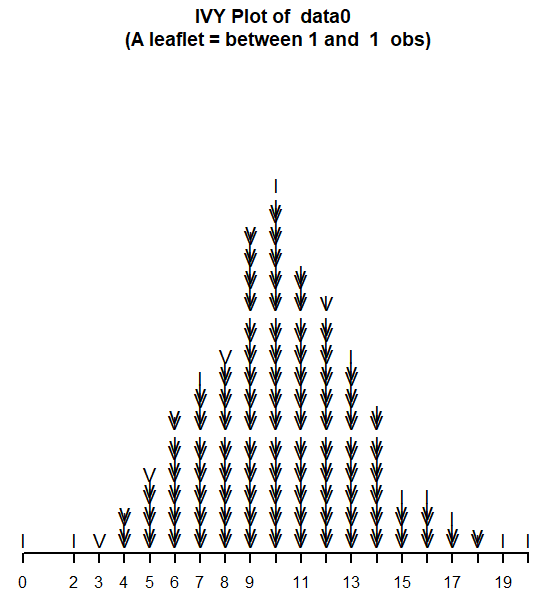
\includegraphics[width=5in,height=4in]{Without_frequency} 

}

\caption[An IVY plot without printing the frequencies]{An IVY plot without printing the frequencies.}\label{fig:unnamed-chunk-1}
\end{figure}
\end{Schunk}

\begin{Schunk}
\begin{figure}[htbp]

{\centering 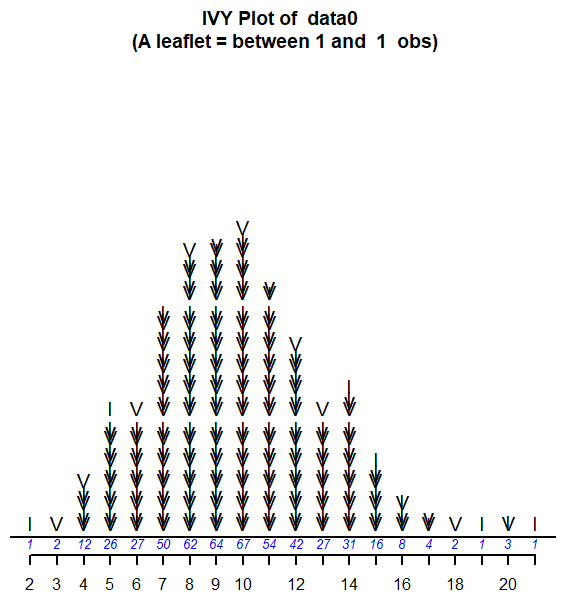
\includegraphics[width=5in,height=4in]{With_frequency} 

}

\caption[An IVY plot with frequencies printed]{An IVY plot with frequencies printed.}\label{fig:unnamed-chunk-2}
\end{figure}
\end{Schunk}

\textcolor{red}{The frequencies are touching the top horizontal line! Like  to see some space there.}

\begin{verbatim}
multiple
\end{verbatim}

The maximum number of observations each leaflet represents. The default
is calculated based on the largest frequency to ensure that at most 20
leaves suffice. Multiple equals the ceiling of one-hundredth of the
maximum frequency.

\begin{verbatim}
delta
\end{verbatim}

The gap between successive values in the data. The default is 1. If the
gap delta is set at 10, for example, any value in the interval {[}5, 15)
will be mapped to 10. Similarly, if the gap is set at 0.1, any value in
the interval {[}1.55, 1.60) will be mapped to 1.5.

\begin{verbatim}
limA
\end{verbatim}

The lower limit of the horizontal axis. The user can choose this limit
if they want to display only those values above this limit. The default
is the minimum value in the data.

\begin{verbatim}
limB
\end{verbatim}

The upper limit of the horizontal axis. The user can choose this limit
if they want to display only those values below this limit. The default
is the maximum value in the data.

\hypertarget{dot-plot-versus-ivy-plot}{%
\subsection{Dot plot versus IVY plot}\label{dot-plot-versus-ivy-plot}}

For a large data set, a dot plot suffers from two drawbacks: the dots
take up too much space; and the dots must be carefully counted to find
out how many numbers are tied at each value. Sarkar and Rashid (2021)
proposed to overcome these drawbacks by drawing an IVY plot: It uses
left, right and vertical notches (leaflets) for each observation, and up
to five notches are joined to form a schematic diagram of one pinnate
compound leaf of an ivy creeper. Thereafter, the notches start afresh,
and the leaves are stacked vertically. To count the leaves fast, a small
extra vertical space is added after every fifth leaf.

Furthermore, the function \texttt{IVYplot} has an option to show the
exact frequency under each vertical stack of leaves. If this option is
enabled, between the leaves and the horizontal axis another horizontal
line is inserted and vertically separated from the horizontal axis to
make room to write the frequencies.

The name ``IVY'' comes from the use of the three upper-case letters I,
V, Y having 1, 2, 2 top endpoints, respectively. Frequencies 1--5 are
indicated as follow: A frequency of 1 is indicated by an I, a frequency
of 2 by a V, a frequency of 3 by staking an I over a V, a frequency of 4
by stacking a Y over a V, and a frequency of 5 by stacking an I over the
symbol for 4. Higher frequencies are formed by stacking enough leaves
vertically, with the topmost leaf possibly having fewer than five
leaflets. For example, a frequency of \(13=2\times 5+3\) is depicted by
stacking two complete leaves with five leaflets and a third leaf with
three leaflets.

If the maximum frequency of 365 is attained at \(x=a\), then to keep the
number of leaves stacked at \(x=a\) under 20, we declare in the subtitle
that each leaflet represents up to 4 observations (since
\(\lceil 365/100 \rceil =4\)), except the topmost leaflet may represent
1, 2, 3, or 4 observations. Then we calculate the number of leaflets at
\(x=a\) to be \(\lceil 365/4\rceil=92\), which we depict by vertically
stacking 18 complete leaves topped by an incomplete leaf consisting of 2
leaflets in the shape of a V. Of course, the same vertical stack can
represent a frequency of 366, 367 or 368. Thus, while all other leaflets
represent 4 observations, (one of) the topmost leaflet represents 1, 2,
3 or 4 observations. Although we could do it, we refrain from shortening
the length of a leaflet to show a lower frequency, since the discrepancy
may be visually imperceptible. Instead, we give the user the option to
print the actual frequencies.

\textcolor{red}{we need a figure to illustrate the above.}

What then do we gain by introducing an IVY plot in the analyst's
toolkit? Given a dot plot, one can read off the exact value of each dot;
however, for a large dataset, tallying the dots stacked at the same
value requires a careful counting and the process is prone to occasional
mistakes. On the contrary, given a frequency histogram, one may read off
the frequencies of the bins from the vertical scale; but one cannot
retrieve the actual values within the bins. Moreover, the distribution
depicted by a histogram depends very much on the choice of the bin
width. An IVY plot merges the advantages of a dot plot and a histogram,
while it simultaneously avoids their drawbacks: It preserves the exact
values and assists in counting the frequencies fast.

\hypertarget{the-ivyplot-package-1}{%
\subsection{The IVYplot Package}\label{the-ivyplot-package-1}}

\begin{verbatim}
if (length(dataCount$x) > 100){
    data0 <- round(data0/delta, 0) * delta
    dataCount <- count(data0)
  }
\end{verbatim}

We wish to permit at most 100 distinct values in the data. Therefore,
values that fall in the same bin given by successive odd multiples of
delta/2 are approximated by the nearest multiple of delta.

\begin{verbatim}
dev.new(width = 12, height = 10)
\end{verbatim}

The function creates a separate window with width 12 and height 10 to
draw an IVY Plot inside.

\begin{verbatim}
dataCount <- count(data0)
\end{verbatim}

The values inside the data given by the user (and thereafter
approximated by a multiple of delta) are counted to produce a frequency
table with distinct values and their frequencies.

\begin{verbatim}
  dataName <- deparse(substitute(data0))
\end{verbatim}

The name of the variable in the user provided data set (if there is a
name) is extracted so that this name can be printed in the title of the
IVY plot.

\begin{verbatim}
  if (length(dataCount$x) > 100){
    data0 <- round(data0/delta, 0) * delta
    dataCount <- count(data0)
  }
\end{verbatim}

If the number of distinct values in the data is greater than 100, the
function will group these values into at most 100 contiguous
subintervals of constant width delta and replace all values within a
subinterval by the midpoint of the subinterval. For example, if delta=1,
then 45.9 and 46.2 will be grouped into subinterval {[}45.5, 46.5) and
then both values will be replaced by 46.

\begin{verbatim}
if (is.null(multiple) == TRUE)
    multiple <- ceiling(max(dataCount$freq)/100)
  for (i in 1:length(dataCount$freq)){
    data1 <- ceiling(dataCount$freq/multiple)
  }
\end{verbatim}

If the user does not input the value of multiple (the number of
observations each leaflet represents), the function will calculate an
appropriate multiple so that at most 20 leaves (or 100 leaflets) will
suffice to represent the frequency at each distinct value, using the
formula ceiling of one-hundredth of the maximum frequency. The function
also saves the new frequency (the ceiling of the ratio when the old
frequency is divided by the multiple) in a separate table. The new
frequencies are used to draw the leaflets; but the old frequencies are
printed underneath the stack of leaves.

\begin{verbatim}
 if (is.null(limA) == TRUE)
    limA = min(mid)
  if (is.null(limB) == TRUE)
    limB = max(mid)
\end{verbatim}

limA and limB are the lower and the upper horizontal limits,
respectively, of the display. If the user does not choose the desired
values for these limits, they automatically default to the minimum and
the maximum values of the data. However, users should specify these
limits if they wish to compare multiple IVY plots drawn in different
panels of the same diagram.

\begin{verbatim}
frame()
  plot.window(xlim = c(limA, limB), ylim = c(-15, maxFreq), xlab = dataName)
  title(main = paste("IVY Plot of ", dataName, "\n (A leaflet = between 1 and ", multiple, " obs)"))
  axis(1, at = c(dataCount$x), lwd = 2, xpd = TRUE)
\end{verbatim}

Draws the frame of the IVY plot, together with a title, a subtitle to
declare the value of the multiple, and the sample size printed at the
top of the plot window.

\begin{verbatim}
  if(showFreq == TRUE){
    lines(c(min(mid) - 2, max(mid) + 2), c(-15, -15), lwd = 2)
  }
\end{verbatim}

If the user chooses to print the frequencies underneath the stacks of
leaves, there will be a new horizontal reference line drawn suficiently
above the horizontal axis so that the frequencies can be printed between
the two lines.

\begin{verbatim}
for (i in 1:length(mid)){
    i1 <- midCount$x[z]
    y <- -16
    if (showFreq == TRUE){
      y <- -12.5
      #if (multiple == 1)
      #y <- -7
    }
    if (leftCount$x[z] < mid[i] && mid[i] < rightCount$x[z]){
\end{verbatim}

This is to check if the original data is within delta/2 of the
``rounded'' data \textcolor{red}{I am not sure of this!}

\begin{verbatim}
      if (data1[z] >= 5){
        times <- data1[z] %/% 5
\end{verbatim}

This determines how many full leaves will be drawn.

\begin{verbatim}
        for (x in 1:times){
          text(i1, y, expression("V"), cex = 1.2, xpd = TRUE)
          y = y + maxFreq/360  #0.05
          text(i1, y, expression("I"), cex = 1.2, xpd = TRUE)
          y = y + maxFreq/90   #0.2
          text(i1, y, expression("v"), cex = 1.5, xpd = TRUE)
          y = y + maxFreq/90   #0.2
          text(i1, y, expression("I"), cex = 1.2, xpd = TRUE)
          if (x %% 5 == 0 && times >= 5)
            y = y + maxFreq/18
          else
            y = y + maxFreq/30   #0.7
          data1[z] = data1[z] - 5
        }
\end{verbatim}

This if/else statement decides if the leaves need to be separated by an
extra space. Atop a string of five full leaves an extra vertical space
is added to expedite counting the leaves.

\begin{verbatim}
      }
      if (data1[z] == 4){
        text(i1, y, expression("V"), cex = 1.2, xpd = TRUE)
        y = y + maxFreq/600 #0.03
        text(i1, y, expression("I"), cex = 0.9, xpd = TRUE)
        y = y + maxFreq/90 #0.2
        text(i1, y, expression("v"), cex = 1.5, xpd = TRUE)
      }
      else if (data1[z] == 3){
        text(i1, y, expression("V"), cex = 1.2, xpd = TRUE)
        y = y + maxFreq/360 #0.05
        text(i1, y, expression("I"), cex = 1.2, xpd = TRUE)
      }
      else if (data1[z] == 2)
        text(i1, y, expression("V"), cex = 1.2, xpd = TRUE)
      else if (data1[z] == 1)
        text(i1, y, expression("I"), cex = 1.2, xpd = TRUE)
\end{verbatim}

After drawing all complete leaves with five leaflets, only one more leaf
with possibly fewer than five leaflets may remain to be drawn. So, we
prefer the if/else if statement is used instead of a loop.

\begin{verbatim}
      if(showFreq == TRUE){
        text(i1, -16, dataCount$freq[z], cex = freqSize, xpd = FALSE, col = "blue", font = 3)
      }
\end{verbatim}

If the user chooses to print the frequencies, then the function will
write the frequencies, with adjustable font size, below the stacks of
leaves.

\begin{verbatim}
      z = z + 1
\end{verbatim}

This z serves as an index to access the vector of rounded values that
will be displayed in the output plot. This is to differentiate from the
vector of the original values that were not rounded. For example: a
vector of rounded values may include (1, 2, 3, 4) but the original
values are (0.8, 0.9, 1, 1.1, 1.9, 2.3,\ldots) The variable z will
account for the displayed value from among (1, 2, 3, 4), and the
variable i will enable the frequency counting within each value.

\hypertarget{summary}{%
\subsection{Summary}\label{summary}}

This article describes how to draw an IVY plot and explains the options
available to the user to modify some default choices. The IVY plot
enhances a dotplot by reducing the space needed to depict large number
of dots and by expediting the count of frequencies. Therefore, an IVY
plot is appropriate for depicting a large data set without distortion.

\hypertarget{references}{%
\subsection{References}\label{references}}

Sarkar, J. and Rashid, M. (2021), IVY Plots and Gaussian Interval Plots,
Teaching Statistics, To appear.

Wilkinson, L. (1999). Dot Plot. The American Statistician, 53(3),
276-281.

\hypertarget{about-this-format-and-the-r-journal-requirements}{%
\subsubsection{About this format and the R Journal
requirements}\label{about-this-format-and-the-r-journal-requirements}}

\texttt{rticles::rjournal\_article} will help you build the correct
files requirements:

\begin{itemize}
\tightlist
\item
  A R file will be generated automatically using \texttt{knitr::purl} -
  see \url{https://bookdown.org/yihui/rmarkdown-cookbook/purl.html} for
  more information.
\item
  A tex file will be generated from this Rmd file and correctly included
  in \texttt{RJwapper.tex} as expected to build \texttt{RJwrapper.pdf}.
\item
  All figure files will be kept in the default rmarkdown
  \texttt{*\_files} folder. This happens because
  \texttt{keep\_tex\ =\ TRUE} by default in
  \texttt{rticles::rjournal\_article}
\item
  Only the bib filename is to modifed. An example bib file is included
  in the template (\texttt{RJreferences.bib}) and you will have to name
  your bib file as the tex, R, and pdf files.
\end{itemize}

\bibliography{RJreferences.bib}

\address{%
Tri Nguyen\\
DePauw University\\%
2 E. Hana Street\\ Department of Computer Science\\ Greencastle, IN 46135 USA\\
%
%
%
\\\href{mailto:tringuyen_2023@depauw.edu}{\nolinkurl{tringuyen\_2023@depauw.edu}}
}

\address{%
Mamunur Rashid\\
DePauw University\\%
2 E. Hana Street\\ Department of Mathematics, Room\\ Greencastle, IN 46135 USA\\
%
\url{http://dpuadweb.depauw.edu/mrashid_web/}%
\\\textit{ORCiD: \href{https://orcid.org/0000-0001-8759-3803}{0000-0001-8759-3803}}%
\\\href{mailto:mrashid@depauw.edu}{\nolinkurl{mrashid@depauw.edu}}
}

\address{%
Jyotirmoy Sarkar\\
Indiana University Purdue University Indianapolis\\%
402 North Blackford Street\\ Indianapolis, IN 46202, USA\\
%
www.math.iupui.edu/\textasciitilde jsarkar%
\\\textit{ORCiD: \href{https://orcid.org/0000-0001-5002-5845}{0000-0001-5002-5845}}%
\\\href{mailto:jsarkar@iupui.edu}{\nolinkurl{jsarkar@iupui.edu}}
}

